
Each of the radionuclide contaminant transport models described in Section
\ref{sec:nuclide_models} capture different combintations of physics present in
the hydrologic contaminant transport problem. To determine how effectively
these physics were captured, single-effect simulations were conducted with
\Cyder and compared to similar analysis \cite{huff_key_2012} conducted with a
more detailed radionuclide transport model, the Clay \gls{GDSM}
\cite{clayton_generic_2011}. The Clay \gls{GDSM} was developed by the \gls{UFD}
Campaign within the \gls{DOE} Office of Nuclear Energy using the GoldSim
simulation environment \cite{golder_associates_goldsim_2010}. Hydrologic
contaminant transport in the Clay \gls{GDSM} relies on the GoldSim contaminant
transport module \cite{golder_associates_goldsim_2010-1}.

These single-effect sensitivity analyses were constructed by repeated
multi-component simulation runs conducted across the valid range for a single
parameter. To verify the behavior of a single parameter of each of the \Cyder
models, one hundred multi-component simulations were conducted, each with a
different value of that parameter.  This parametric analysis was conducted to
show that, for an arbitrary isotope, the expected dependence on that parameter
is captured. In the case of real isotopes in a full simulation, the same model
will be invoked with real parameters for each isotope. Thus, the this model
agreement is representative in all cases.

The results acheived with \Cyder were compared to the results of a similiar
parametric sensitivity analysis using the Clay \gls{GDSM} which was reported in
\cite{huff_key_2012}.

\subsubsection{Solubility Sensitivity}
Each of the radionuclide contaminant transport models described in Section
\ref{sec:nuclide_models} capture different combintations of physics present in
the hydrologic contaminant transport problem. To determine how effectively
these physics were captured, single-effect simulations were conducted with
\Cyder and compared to analysis was conducted with a more detailed radionuclide
transport model, the Clay \gls{GDSM} \cite{clayton_generic_2011}. The Clay
\gls{GDSM} was developed by the \gls{UFD} Campaign within the \gls{DOE} Office
of Nuclear Energy and relies on the GoldSim simulation environment
\cite{golder_associates_goldsim_2010} and its contaminant transport module
\cite{golder_associates_goldsim_2010-1}.

These single-effect sensitivity analyses were constructed by repeated
multi-component simulation runs conducted accross the valid range for a single
parameter.

To verify the behavior of the solubility limitation model in the Mixed Cell
model, for example, one hundred multi-component simulations were conducted,
each with a different reference solubility limit. This parametric analysis was
conducted to show that, for an arbitrary isotope, the expected solubility
limitation behavior is captured. In the case of real isotopes in a full
simulation, the same model will be invoked with real parameters for each
isotope. Thus, the this model agreement is representative in all cases.

The results acheived with \Cyder were compared to the results of a parametric
sensitivity analysis using the Clay \gls{GDSM} reported in
\cite{huff_key_2012}. That analysis showed that for solubility limits below a
certain threshold, the dose releases were directly proportional to the
solubility limit, indicating that the radionuclide concentration saturated the
groundwater up to the solubility limit near the waste form.  For solubility
limits above the threshold, however, further increase to the limit had no
effect on the peak dose. This demonstrates the situation in which the
solubility limit is so high that even complete dissolution of the waste
inventory into the pore water is insufficient to reach the solubility limit.

\begin{figure}[ht]
\begin{center}
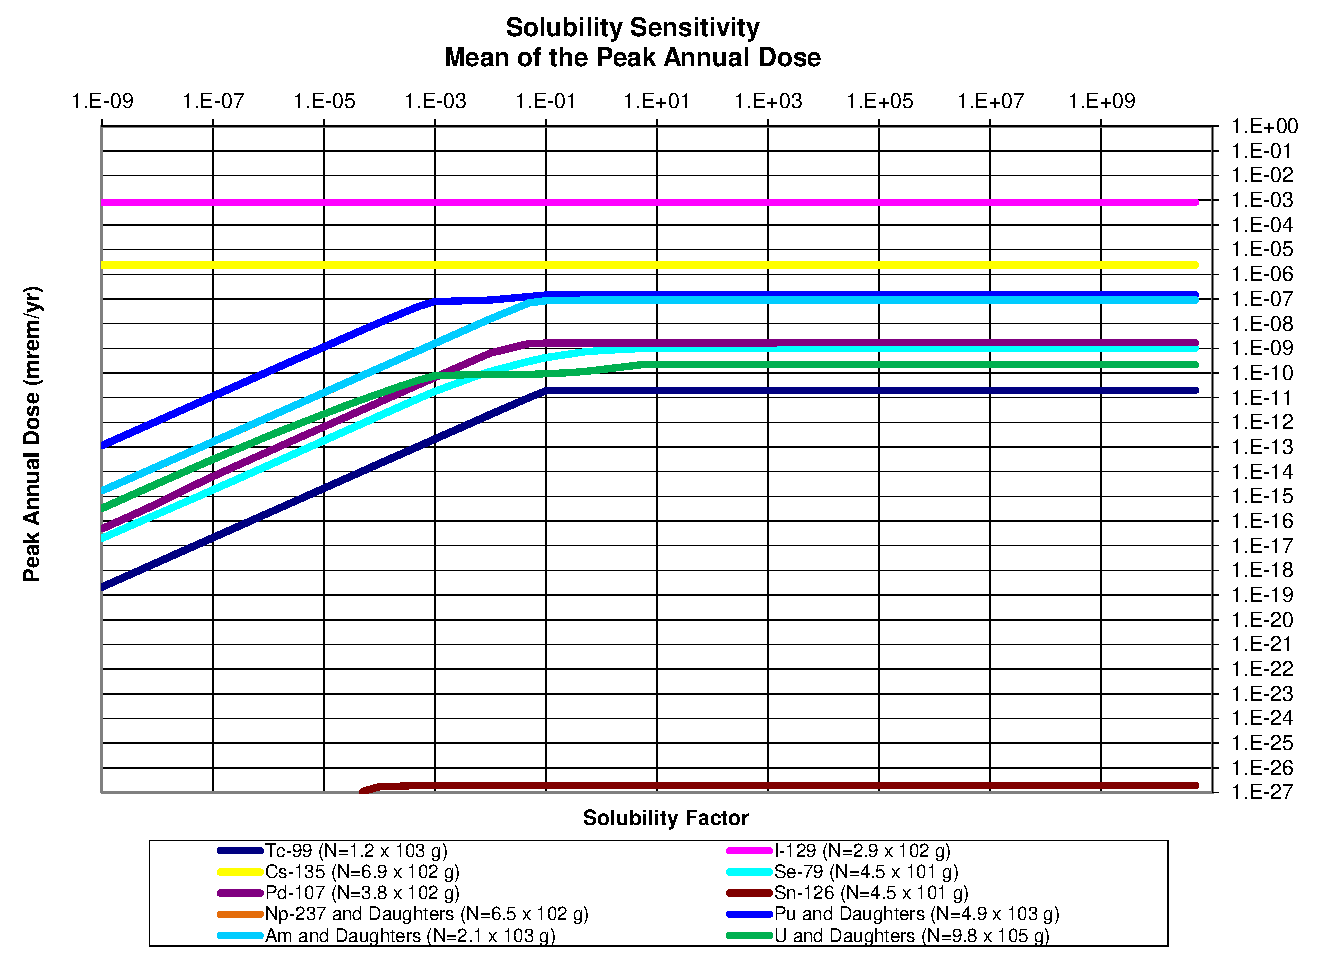
\includegraphics[width=0.7\linewidth]{./results/images/Solubility_Summary_SolFactor.eps}
\caption[Solubility factor sensitivity in GDSM Clay model]{Solubility factor sensitivity. The peak annual dose due to an inventory, $N$, of each isotope. This result was acheived with a parametric analysis using a detailed model of a generic clay repository \ref{huff_key_2012}}
\label{fig:SolSumFactor}
\end{center}
\end{figure}

\begin{figure}[ht]
\begin{center}
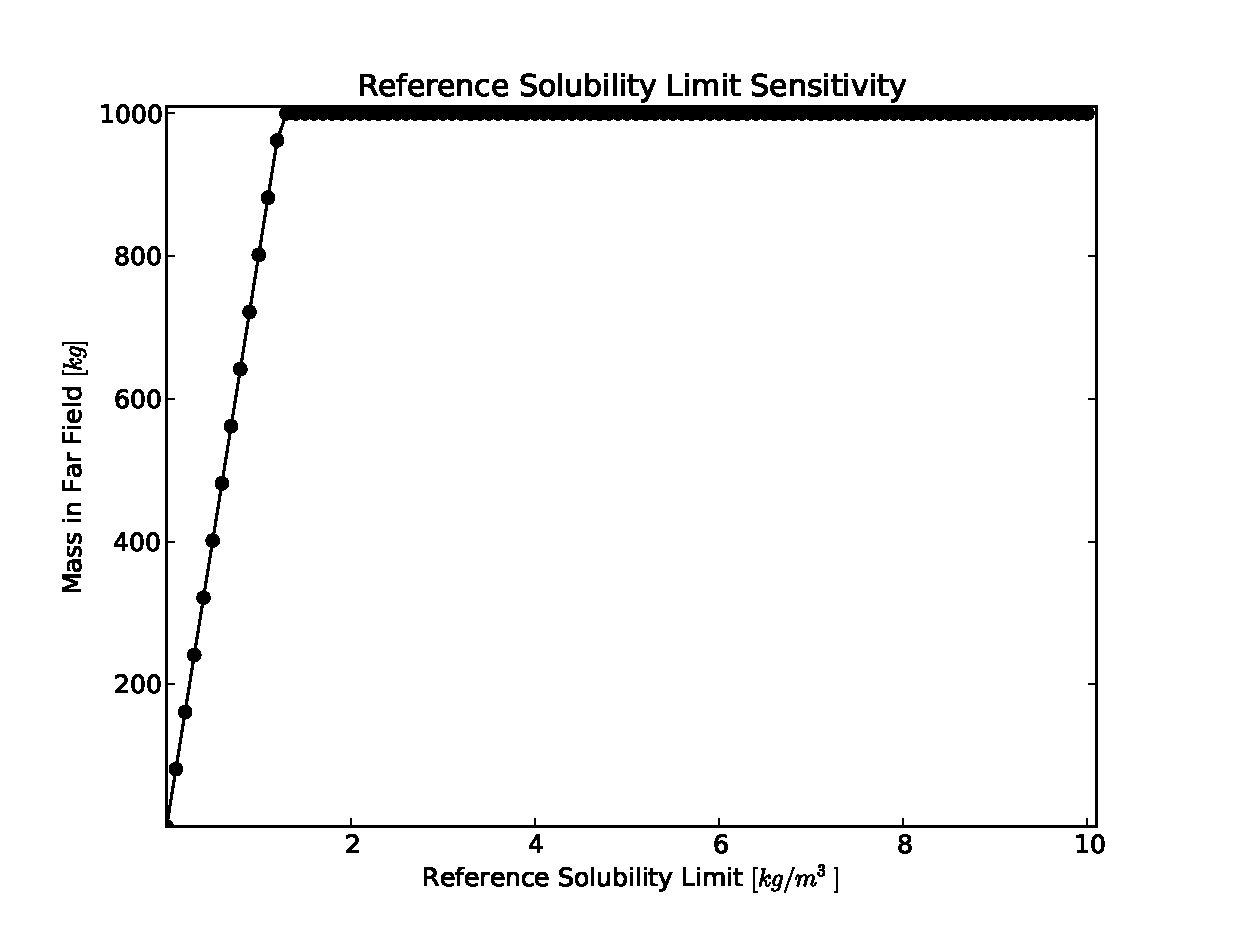
\includegraphics[width=0.7\linewidth]{./results/images/sol.eps}
\caption[Solubility Sensitivity in the Mixed Cell Model]{Sensitivity demonstration of solubility limitation in \Cyder for an arbitrary isotope assigned a variable solubility limit.}
\label{fig:sol_result}
\end{center}
\end{figure}


The results in Figure \ref{fig:SolSumFactor}, from the detailed parametric
analysis in \cite{huff_key_2012}, it is clear that for
solubility constants lower than the saturation threshold, the transport regime is solubility
limited and the relationship between peak annual dose and solubility limit is
strong.  Above the threshold, the transport regime is inventory limited
instead.

In the corresponding parametric analysis of \Cyder performance, it was shown that the
solubility sensitivity behavior closely matched that of the \gls{GDSM}
sensitivity behaviors. Specifically, in Figure \ref{fig:sol_result}, a sharp turnover
is seen where the solubility limit exceeds the point at which it limits
movement. For increased solubility limits, release remains constant, as
expected.

%\begin{figure}[ht]
%\begin{center}
%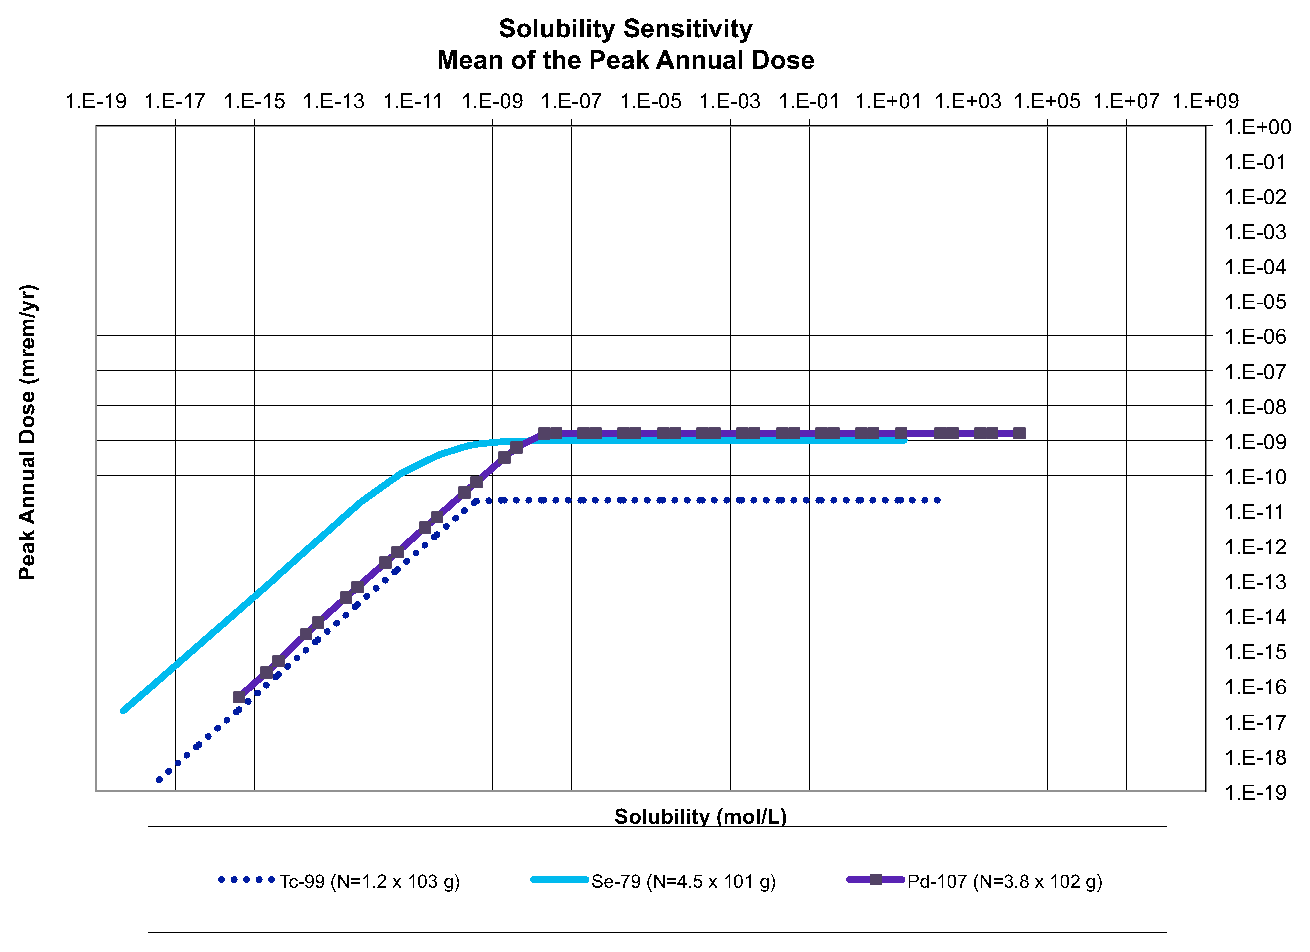
\includegraphics[width=0.7\linewidth]{./results/images/Solubility_Summary_Sol.eps}
%\caption[Solubility limit sensitivity in GDSM Clay model]{Solubility limit sensitivity. The peak annual dose due to an inventory,
%$N$, of each isotope.}
%\label{fig:SolSum}
%\end{center}
%\end{figure}


\FloatBarrier
\subsubsection{Sorption Sensitivity}



As the distribution coefficient $K_d$ increases, so does the retardation 
coeffcient $R_f$, according to the relation $R_f = 1+ \rho_b\frac{K_d}{\theta}$. As these two values increase, contaminants tend 
toward the solid phase. An increase in these coefficients, then, has the effect 
of limiting dissolved concentration.

In the parametric sensitivity analysis reported in \cite{huff_key_2012},
the expected inverse relationship between the retardation factor and resulting
peak annual dose was found for all elements except $^{129}I$ and $^{79}Se$. 
These two isotopes have effectively no solubility limit and therefore
demonstrate no sensitivity whatsoever to a the solubility limit multiplication 
factor. In the low retardation coefficient cases, a regime is established in 
which the peak annual dose is entirely unaffected by changes in retardation 
coefficient.

For large values of retardation coefficient, the sensitivity to small changes
in the retardation coefficient increases dramatically. In that sensitive
regime, the change in peak annual dose is inversely related to the retardation
coefficient. Between these two regimes was a transition regime, in which the
$K_d$ factor ranges from $1\times10^{-5}$ to $5\times10^{0} [-]$.

It is clear from Figure \ref{fig:KdSumFactor} that
for retardation coefficients greater than a threshold, the
relationship between peak annual dose and retardation coefficient is a strong
inverse one.

\begin{figure}[ht]
\centering
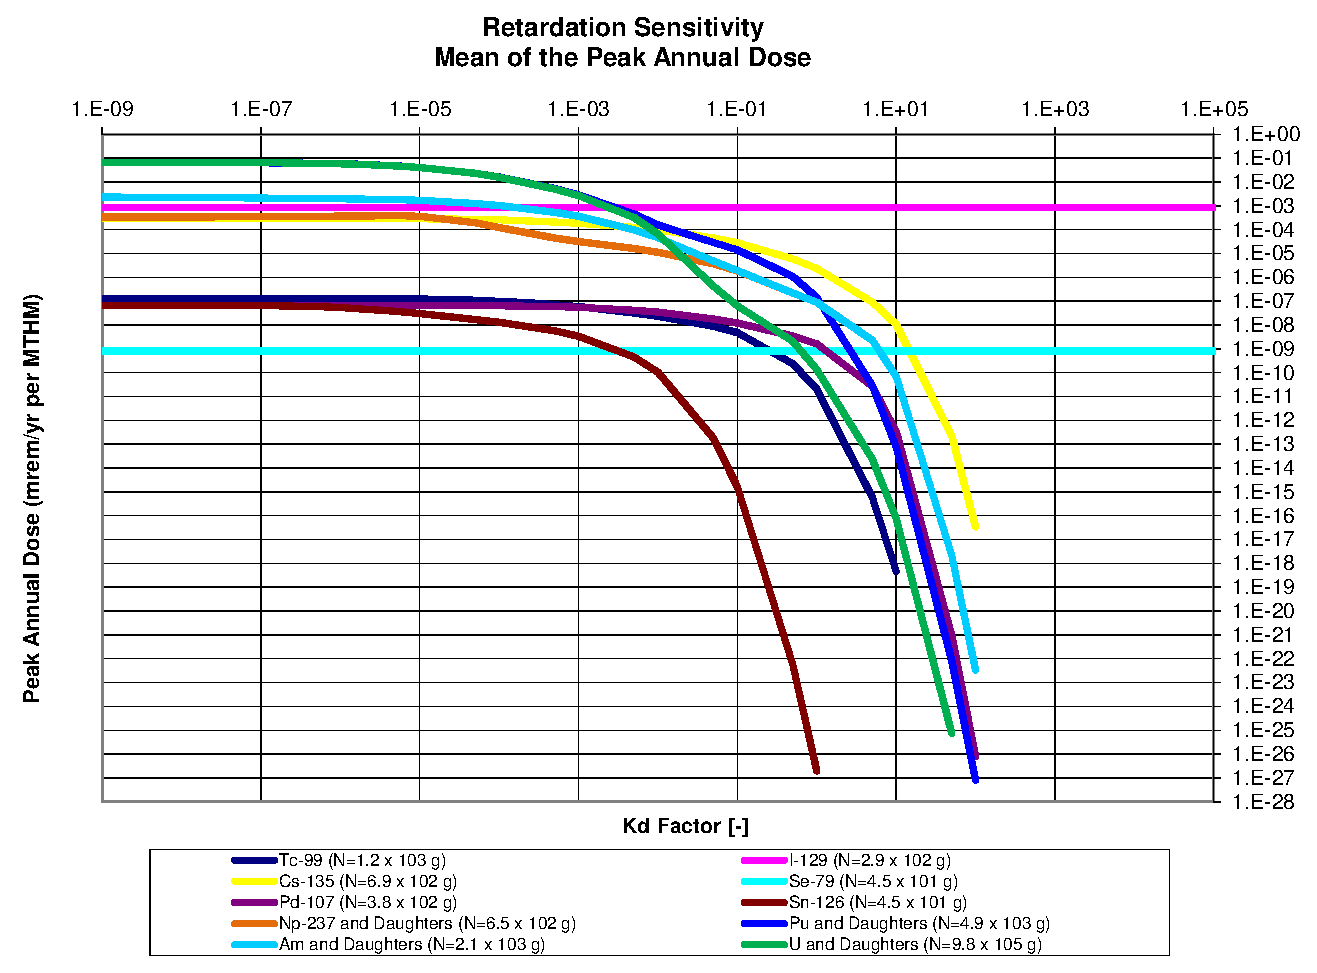
\includegraphics[width=0.7\linewidth]{./results/images/Retardation_Summary_kdFactor.eps}
\caption[$K_d$ factor sensitivity in Clay GDSM]{$K_d$ factor sensitivity in 
        DOE Clay GDSM, reproduced from \cite{huff_key_2012}.
The peak annual dose due to an inventory,
$N$, of each isotope.}
\label{fig:KdSumFactor}
\end{figure}

\FloatBarrier


In the parametric analysis of \Cyder performance, it was shown that sorption
sensitivity behavior closely matched that of the \gls{GDSM} sensitivity
behaviors. Specifically, in Figure \ref{fig:kd_result}, increasing the retardation
coefficient results in a smooth but dramatic turnover.

\begin{figure}[ht]
\centering
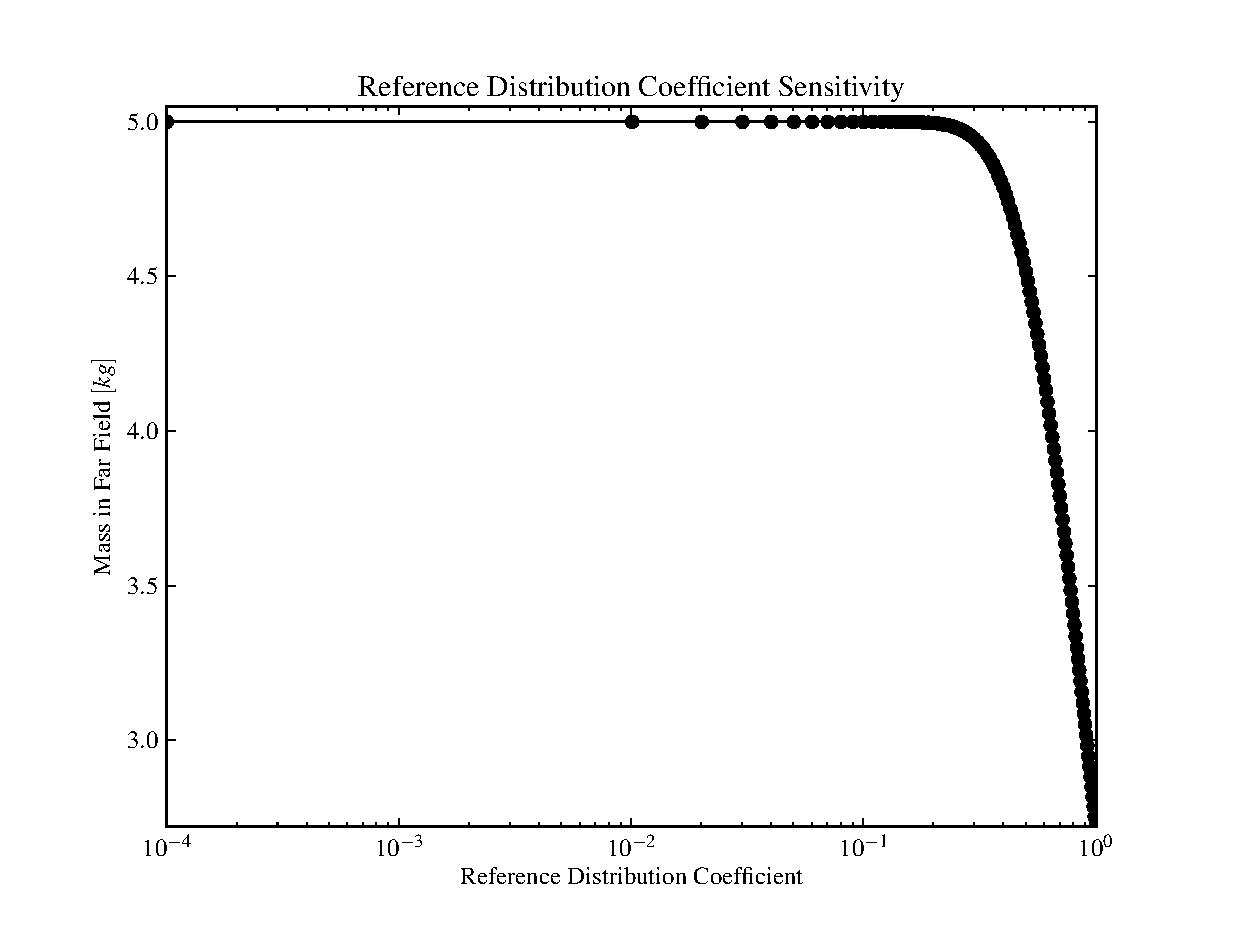
\includegraphics[width=0.7\linewidth]{./results/images/kd.eps}
\caption[$K_d$ sensitivity in the Mixed Cell Model]{$K_d$ sensitivity in the
\Cyder tool for an arbitrary isotope assigned a variable $K_d$ coefficient.}
\label{fig:kd_result}
\end{figure}


\FloatBarrier
\subsubsection{Waste Form Degradation Rate Sensitivity}
In the parametric sensitivity analysis reported in \cite{huff_key_2012}
\ref{sec:wfdeginv}, the results showed two regimes. In the first regime, the
mean of the peak annual dose rates is directly proportional to both the mass
factor (an inventory mass multiplier) and the fractional waste
form degradation rate. For some radionuclides, attenuation occurs for high
values of both parameters as the release of radionuclides is limited by
dispersion parameters. This phenomenon can be seen in the figures below in which
transition between regimes for higher degradation rates happens at lower mass
factors than transition between regimes for lower degradation rates.

The peaks for highly soluble, non-sorbing elements such as $I$ and $Cl$
are directly proportional to mass factor for most
values of waste form degradation rates. This effect can be seen in Figures
\ref{fig:WFDegI129} and \ref{fig:WFDegCl36}.


Highly soluble and non-sorbing $^{129}I$ demonstrates a direct proportionality between dose rate and
fractional degradation rate until a turnover where other natural system
parameters dampen transport.

\begin{figure}[ht!]
\begin{minipage}[b]{0.45\linewidth}
\centering
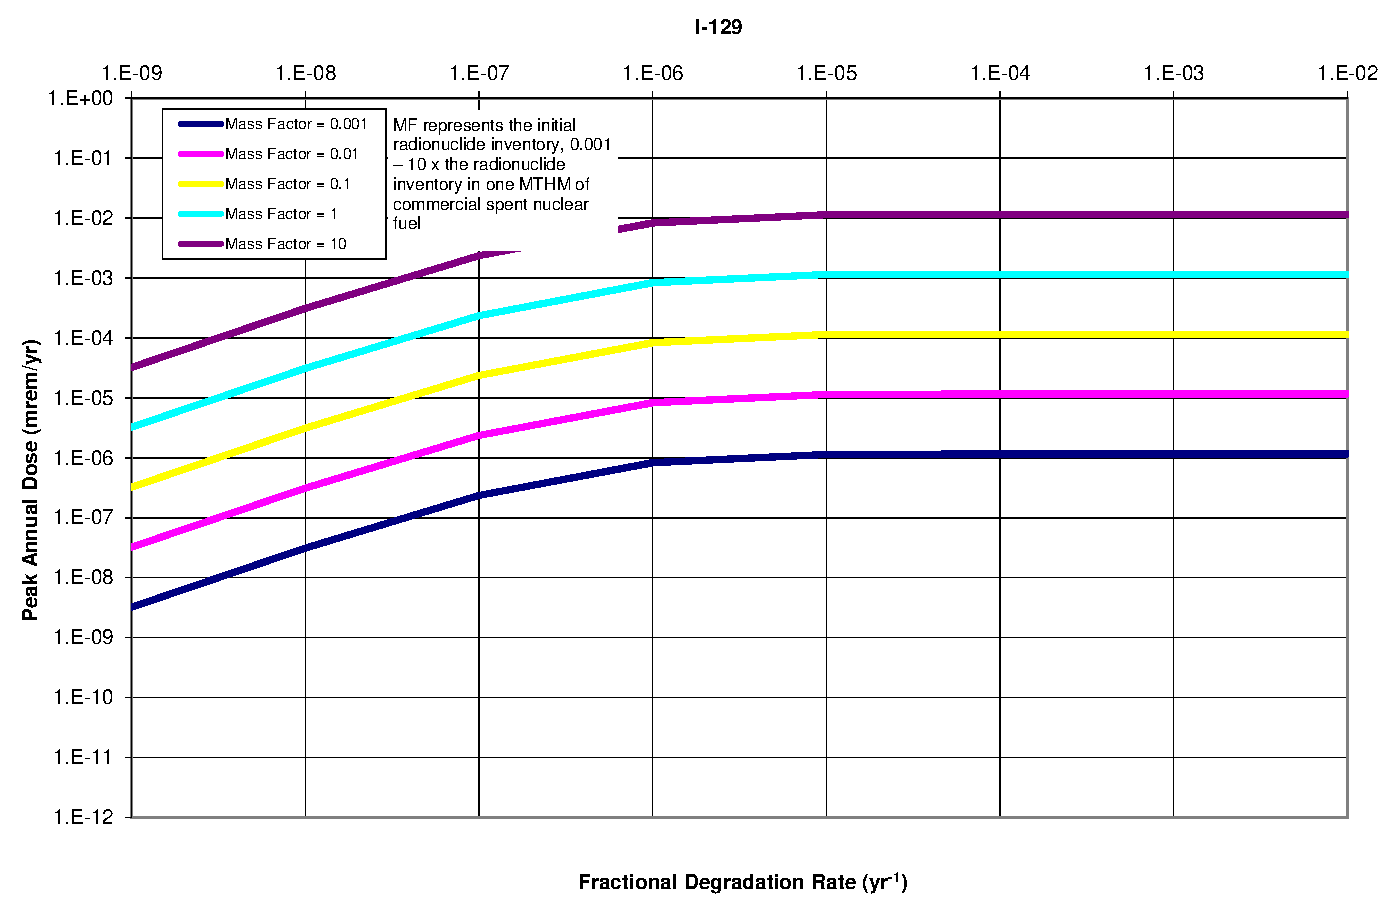
\includegraphics[width=\linewidth]{./results/images/WFDegAndInv/I-129.eps}
\caption{$^{129}I$ waste form degradation rate sensitivity.}
\label{fig:WFDegI129}

\end{minipage}
\hspace{0.05\linewidth}
\begin{minipage}[b]{0.45\linewidth}

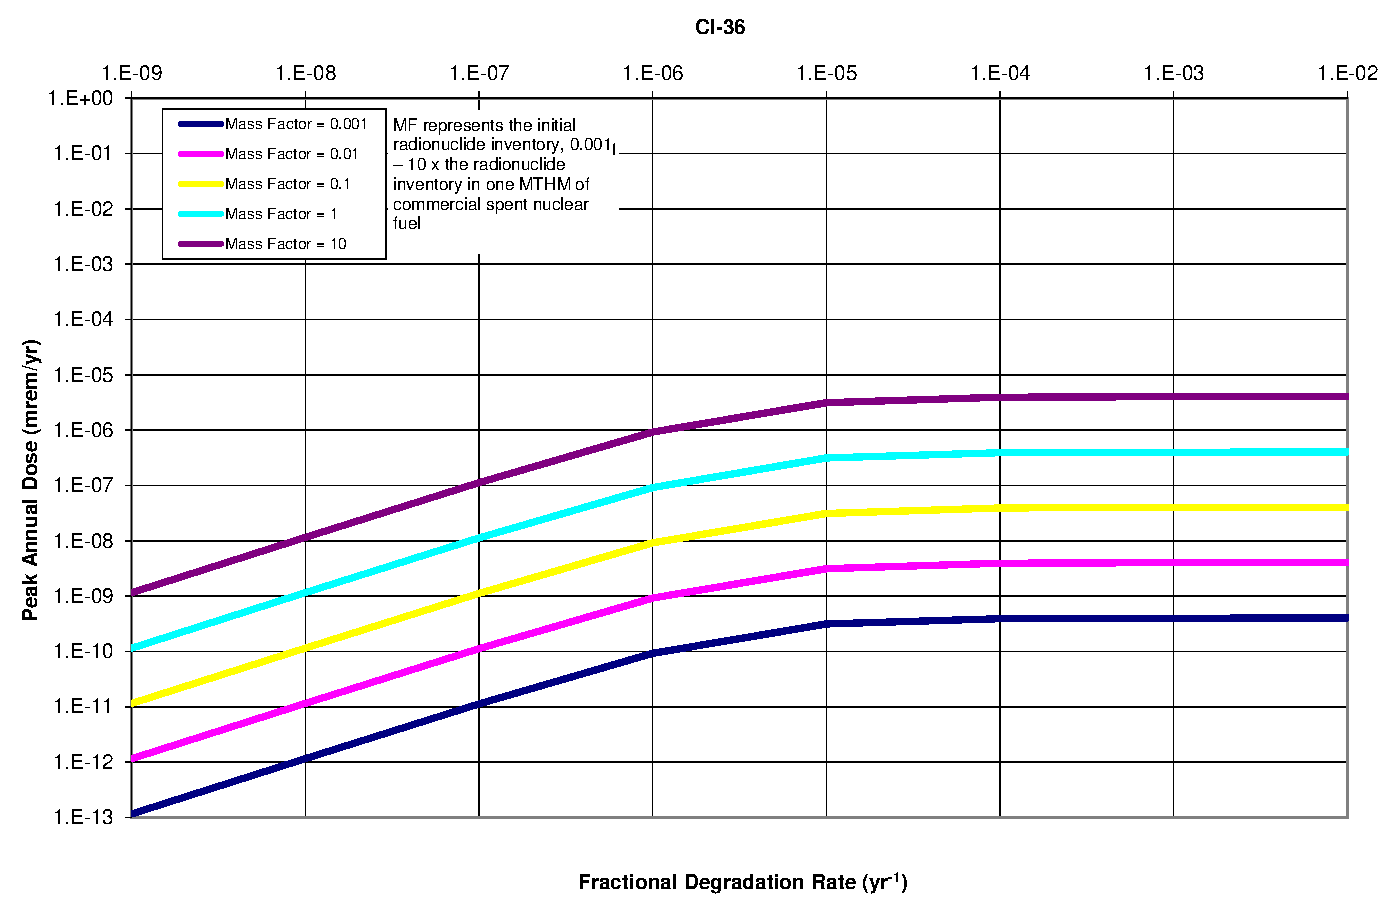
\includegraphics[width=\linewidth]{./results/images/WFDegAndInv/Cl-36.eps}
\caption{$^{36}Cl$ waste form degradation rate sensitivity.}
\label{fig:WFDegCl36}
\end{minipage}
\end{figure}

\FloatBarrier


In the parametric sensitivity analysis conducted with the \Cyder tool, waste
form degradation rate sensitvity similarly shows the two regimes noted in the
\gls{GDSM} analysis.

\begin{figure}[htbp!]
\begin{center}
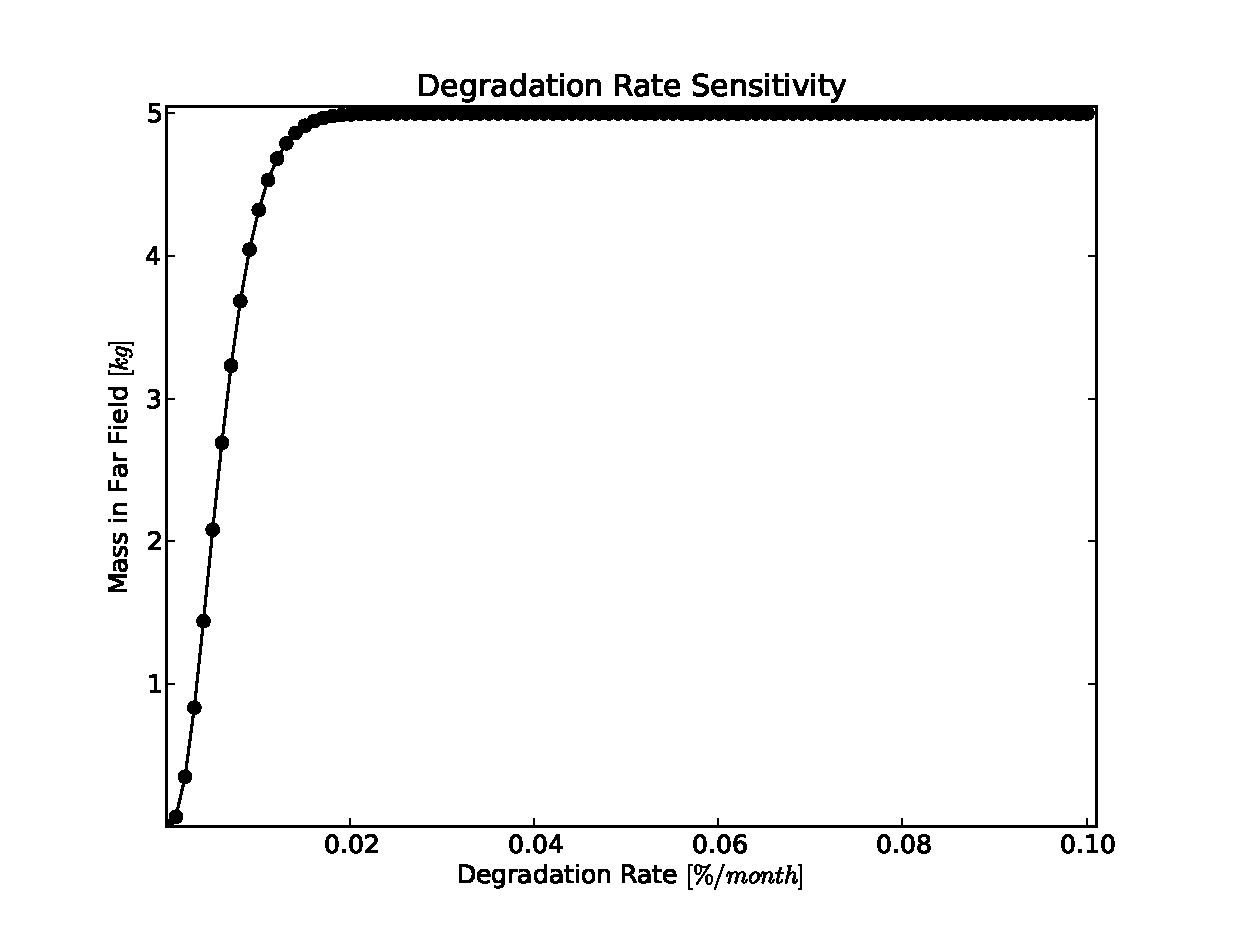
\includegraphics[width=0.7\linewidth]{./results/images/WFDegAndInv/deg.eps}
\end{center}
\caption{Sensitivity demonstration of the degradation rate in \Cyder for an
arbitrary isotope.}
\label{fig:deg}
\end{figure}


\FloatBarrier
